\documentclass{article}
\usepackage{graphicx} % Required for inserting images
\usepackage{amsmath,amsfonts,amssymb,dsfont}
% \usepackage[french]{babel}
\usepackage[english]{babel}
\usepackage{lmodern}
\usepackage{lastpage}
\usepackage{float}
\usepackage{caption}
\usepackage{subcaption}



\title{Research on High Precision Solution of Goddard Problem}
\author{Lechuan ZHOU, François PACAUD}
\date{February 2025}

\begin{document}

\maketitle

\newpage
\tableofcontents
\clearpage


\section{Introduction}
This research focus on improving the precision of numerical solutions of Goddard problem with Julia built-in optimization solvers. In this section, we present an introduction over the problem to study and the applied methodology in this research. Related researches are also presented at the end. 
\subsection{Goddard problem}
\label{sec:GoP}
The Goddard problem, first proposed by Robert H. Goddard in 1919\cite{A method of reaching}, is an optimal control problem in the field of aerospace engineering. This problem aims to maximize the final height of a rocket by modifying its thrust over time, which is considered as an input vector of control of the system. Its mathematical description is as follows:
\begin{align*}
\max \ &h(t_{f}) \\
s. \ t. \ & \dot{h}(t) = v(t) \\
& \dot{v}(t) = \frac{u(t)-D(v,h)}{m(t)}-g(h) \tag{1.1}\\
& \dot{m}(t) = -\frac{u(t)}{c} \\
& 0 \le u(t) \le u_{max}
\end{align*} 
where $h$,$v$,$m$ represent respectively the height, the vertical velocity and the mass of the rocket in function of time. $D$ represents a force of drag in function of height and vertical velocity. $g$ represents the gravity in function of height. The $u$($T$ in other versions) is the generated thrust, which is treated as a bounded input control.

As is presented in the equation (1.1), the Goddard problem is a nonlinear optimal control problem, where several challenges, especially the existence and optimality of solution, arise when seeking numerical solutions. In order to obtain an optimal solution with reasonable computing power, specific solving methods and algorithms are developped and applied in today's numerical solvers, which is elaborated in section \ref{sec:NuS}.

Furthermore, the Goddard problem is famous for containing a singular arc, causing a need of extra criteria to converge to an optimal solution, which is elaborated in section \ref{sec:Sing}.

To be specific, this research focus on improving the quality, which equals to precision, of Goddard problem's solution without adding the cost of computational resources.

\subsection{Numerical solutions for nonlinear optimal control}
\label{sec:NuS}
A general definition of nonlinear optimal control(OC) problem is as follows:
\begin{align*}
    \min_u \ &c(x,u) \\ s.t.\ &g(x,u)=\mathbf{0}\\ &\mathcal{L}=c(x,u)-\lambda^T g(x,u) \\ & G = \nabla g(x,u)
\end{align*}
where $g$ refers to equality constraints, $\lambda$ Lagrangian multipliers and $G$ Jacobian of equality constraints.

Unlike linear optimization and quadratic optimization, numerically solving a nonlinear OC problem requires specific approaches. Main solution approaches can be classified in two fields: direct methods and indirect methods\cite{Betts}.

Indirect methods use Pontryagin's minimum principle to reduce the problem to boundary value differential equations, offering high precision but requiring good initial estimates. Direct methods, by contrast, discretize the problem to obtain a finite-dimensional nonlinear optimization problem that can be solved using established algorithms. These direct methods provide greater robustness but typically achieve lower precision, particularly when solved using interior point algorithms where the active set is determined with limited precision (typically $10^{-8}$).
Due to this precision limitation, it's common practice to refine solutions from direct methods using indirect methods in a two-stage approach. 

This research aims to develop a direct method to obtain high-quality solutions and reduce used computational resources at the same time. Direct methods generally discretize the continuous state functions $x$ (e.g. height, velocity, mass) to their respective value at each geven moment. Which means instead of analysing $x: t\in \mathbb{R}\rightarrow X\in\mathbb{R}_{n_x}$, direct methods focus on discretized states $x=\left[x_1,x_2,\cdots,x_{nh}\right]\in \mathbb{R}_{n_x \times nh}$, where $nh$ refers to the number of discretisation. 

To achieve an optimal objective by using nonlinear solvers, the following conditions, named Second order sufficient condition(SOSC) and Linear independent constraint qualification(LICQ) are necessary to be satisfied:

\begin{itemize}
    \item SOSC: The reduced Hessian is positive definite or negative definite to achieve minimum or maximum solutions. In another word, the eigenvalues of $Z^TWZ$ should be all positive or all negative, where $W=\nabla^2\mathcal{L}$ and $GZ=0$. 
    \item LICQ: The Jacobian of equality constraints should be of full rank, which means that all columns of $G$ are linearly independent.
\end{itemize}

\subsection{Singular arcs in optimal control problems}
\label{sec:Sing}
In optimal control problems, the extrem solutions (maximum or minimum) are obtained where the first derivative of Hamiltonian $H$ by control $u$ is zero, which are called extremal arcs\cite{Bryson}. In cases where the extremal arcs occur only on which the Hessian of Hamiltonian by $u$, $H_{uu}$, is singular, such arcs are called singular arcs. The situations that $H_{uu}$ is neither definite positive nor definite negative indicates that additional criteria should be added to determine whether the model is optimizing or not on a singular arc.

Take the Goddard problem as an example, the Hamiltonian of of the system discribed in section \ref{sec:GoP} is 
\[
H = \lambda_h v+ \lambda_v (\frac{u-D}{m}-g)- \lambda_m \frac{u}{c} \tag{1.2}
\]

The first and second derivative of $H$ by the control $u$ are
\[
H_u = \frac{\lambda_v}{m}-\frac{\lambda_m}{c} ,\quad H_{uu}=0 \tag{1.3}
\]
(1.3) shows that the extremal arcs, which are supposed to be possible optimal solutions, always coincide with singular arcs. Furthermore, according to equation (1.2), to maximize $H$ with respect to $u$ is equal to maximize
\[
(\frac{\lambda_v}{m}-\frac{\lambda_m}{c})u
\]

The three possible solutions of Goddard problem are then 

\begin{align*}
    F &= F_{max}  \qquad \text{if} \ \frac{\lambda_v}{m}-\frac{\lambda_m}{c}>0 \\
    0 &< F < F_{max} \qquad \text{if} \ \frac{\lambda_v}{m}-\frac{\lambda_m}{c}=0 \\
    F &= 0 \qquad \text{if} \ \frac{\lambda_v}{m}-\frac{\lambda_m}{c}<0
\end{align*}

The above solutions show that the optimal control follows a ``bang-arc-bang'' trend, which starts with the maximum thrust and ends with zero.


\clearpage

\section{Methods}
In this section, we present the methods employed to solve the Goddard problem through numerical optimization techniques. Our approach combines julia optimization models with established discretisation schemes and selected test parameters to ensure robust and accurate solutions.

\subsection{Julia-based model of optimization}
Julia programming language is selected as computational platform for this research due to the following advantages:
\begin{itemize}
    \item \textbf{Efficiency and readability}: Julia uses just-in-time compilation, which enables C-like performance while keeping its Python-like readabilit. This characteristic is critical for computationally intensive optimization problems to be modelized and solved.
    \item \textbf{JuMP.jl}: JuMP, an open-source julia library offers a unified framework to multiple solvers, allowing numerical experimentation with different optimizers including IPOPT, KNITRO, and NLopt.
    \item \textbf{Automatic Differentiation}: Julia's ForwardDiff.jl and ReverseDiff.jl packages compute exact gradients and Jacobians automatically, which improves accuracy and convergence rates.
\end{itemize}

In this research, we mainly use the function JuMP.Model to build optimization models of Goddard problem, where the dynamique and schemes of discretisation are treated as equality and inequality constraints of the model.
\subsection{Realized schemes of discretisation}
As is discussed in section \ref{sec:NuS}, the continuous optimal control problem must be transformed into an adaptable discrete form for numerical optimization. In this section, we present the different schemes of discretisation as equality constraints, where $h$ is the time between two discretised moments, $\textbf{y}_k$ and $\textbf{u}_k$ are the vector of state and control at $k$-th discretised moment, $\textbf{f}$ is the dynamics and $\textbf{f}_k$ the dynamics of system at $k$-th discretised moment. The discretisation schemes realized in this research are as follows:

\begin{itemize}
    \item \textbf{Explicit Euler's Method}: 
\begin{align*}
    \textbf{y}_{k+1} = \textbf{y}_k + h \textbf{f}_k
\end{align*}
    \item \textbf{Implicit Euler's Method}:
\begin{align*}
    \textbf{y}_{k+1} = \textbf{y}_k + h \textbf{f}_{k+1}
\end{align*}
    \item \textbf{Trapezoidal Collocation}: 
\begin{align*}
    \textbf{y}_{k+1} = \textbf{y}_k + \frac{h}{2} (\textbf{f}_k+\textbf{f}_{k+1})
\end{align*}
    \item \textbf{Hermite-Simpson Collocation}: 
\begin{align*}
    \textbf{y}_{k+1} = \textbf{y}_k + \frac{h}{6} (\textbf{f}_k+4\bar{\textbf{f}}_{k+1}+\textbf{f}_{k+1})
\end{align*}
where 
\begin{align*}
    \bar{\textbf{y}}_{k+1} &= \frac{1}{2}(\textbf{y}_k+\textbf{y}_{k+1}) + \frac{h}{8}(\textbf{f}_k -\textbf{f}_{k+1} ) \\
    \bar{\textbf{f}}_{k+1} &= \textbf{f}(\bar{\textbf{y}}_{k+1},\textbf{u}_{k+1},h)
\end{align*}
\end{itemize}

These schemes of discretisation are used to obtain the best performance with every set of parameter as well as to verify the theoretical conclusions, which should be irrelevant of the chosen scheme. 

\subsection{Parameters to finetune the model}
To improve the quality of obtained solutions and to observe the behavior of optimizing models, two parameters, $nh$ and $tol$, are introduced and set changeable for each optimizing model. $nh$ represents the number of discretisation and $tol$ represent the function tolerance of optimization model, which bounds the minimum change of the objective function between two iterations. 

Other parameters, e.g. initial mass $m_0$, coefficient of drag $c$, maximum thrust $u_{max}$, are set identical in different models.

In section \ref{sec:Imp}, another parameter $w_{obj}$ is also introduced to balance the weight between optimizing the target function and optimizing the integrated residuals
\clearpage

\section{Results and Discussion}
In this section, we present different solutions obtained with numerical solvers and schemes of discretisation discussed above. To set a standard, here we present a solution as``Theoretical optimal solution" to demonstrate how close other solutions are to the optimal one. 

\begin{figure}[ht]
    \centering
    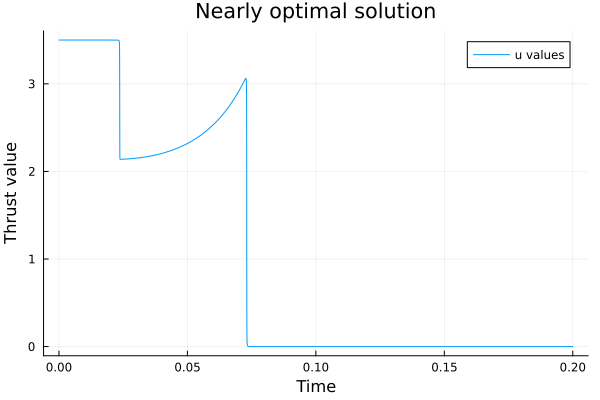
\includegraphics[width=0.9\textwidth]{Nearly Optimal.png}
    \caption{\label{fig:opt} One of the most accurate solutions with costly computational resource, serving as a reference of ``Theoretical optimal solution", where the ``bang-arc-bang'' trend is well presented}
\end{figure}

\subsection{Results of numerical solutions}
In this section, we present the numerical solutions obtained within considerable cost of calculation power (limited iterations and $nhs$), in order to compare the common role played by $nh$ and $tol$ in numerical optimization models. The influence of singular arcs discussed in section \ref{sec:Sing} are also presented and generalized

The default initial parameters and constraints are set as follows: $h(0)=1.0, v(0)=0.0, m(0)=1.0, m(t_f)=0.0, g(h_0)=1.0, c = 0.5$. To first have a general idea on cost of calculation power ($nh$), we calculated the performance of each scheme of discretisation with default tolerance $tol = 10^{-8}$. The results are presented in Figure \ref{fig:defaulttol}
\begin{figure}[ht]
    \centering
    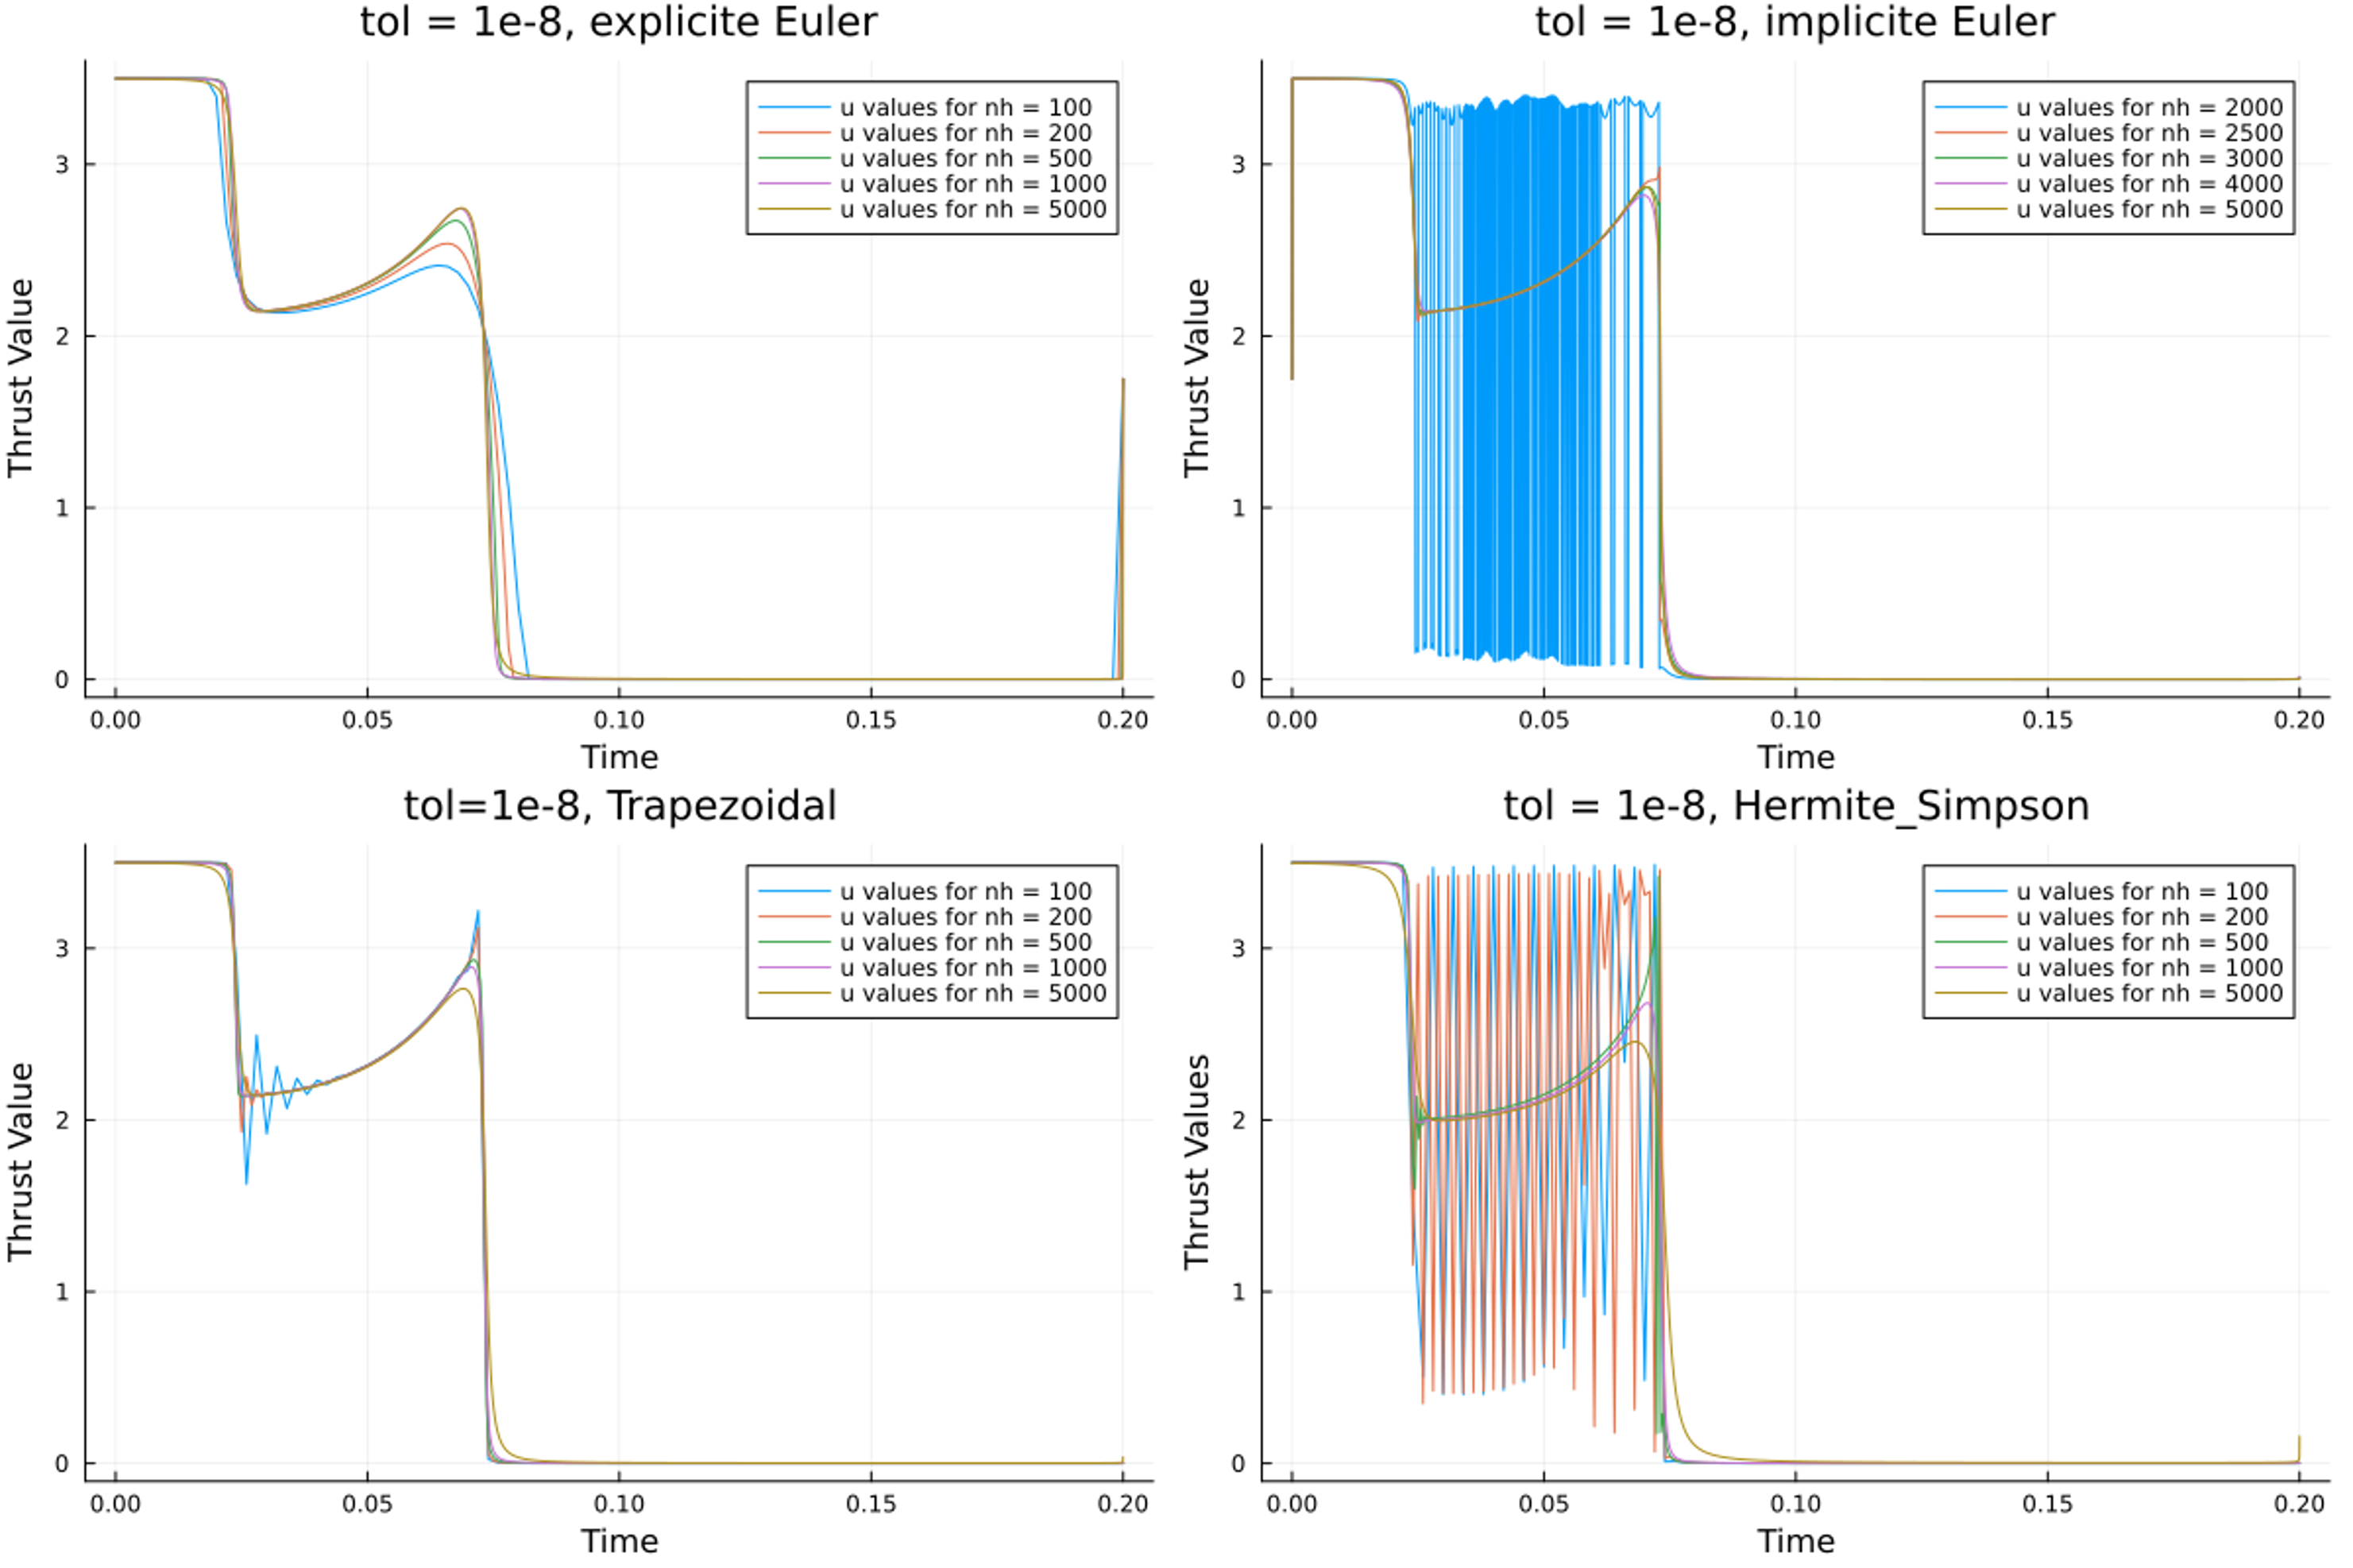
\includegraphics[width = \textwidth]{default tol.png}
    \caption{\label{fig:defaulttol} The calculated numerical solutions by different schemes of discretisation. Tolerances are set to $10^{-8}$ and $nh$ vary from 100 to 5000.}
\end{figure}

As is presented in Figure\ref{fig:defaulttol}, two common trends of numerical solutions are in all those four results: First, fluctuations are obesrved on the singular arc of all solutions except for explicit Euler scheme. These fluctuations tend towards smooth curves with the increase of $nh$. Second, compared with the theoretical optimal solution, the peak between 0.05s and 0.1s has been significantly reduced and smoothened, especially when it comes to a high $nh$.

According to the obtained results, the curves with $nh = 500$ are generally acceptable as solutions with neither many fluctuations nor over-smoothing of the peak at the end of the singular arc (except for implicit Euler, where such curve is obtained with $nh = 2500$). The following comparisons between tolerances $tol$ presented on Figure \ref{fig:acceptnh} are based on the corresponding acceptable number of discretisation.

\begin{figure}[ht]
    \centering
    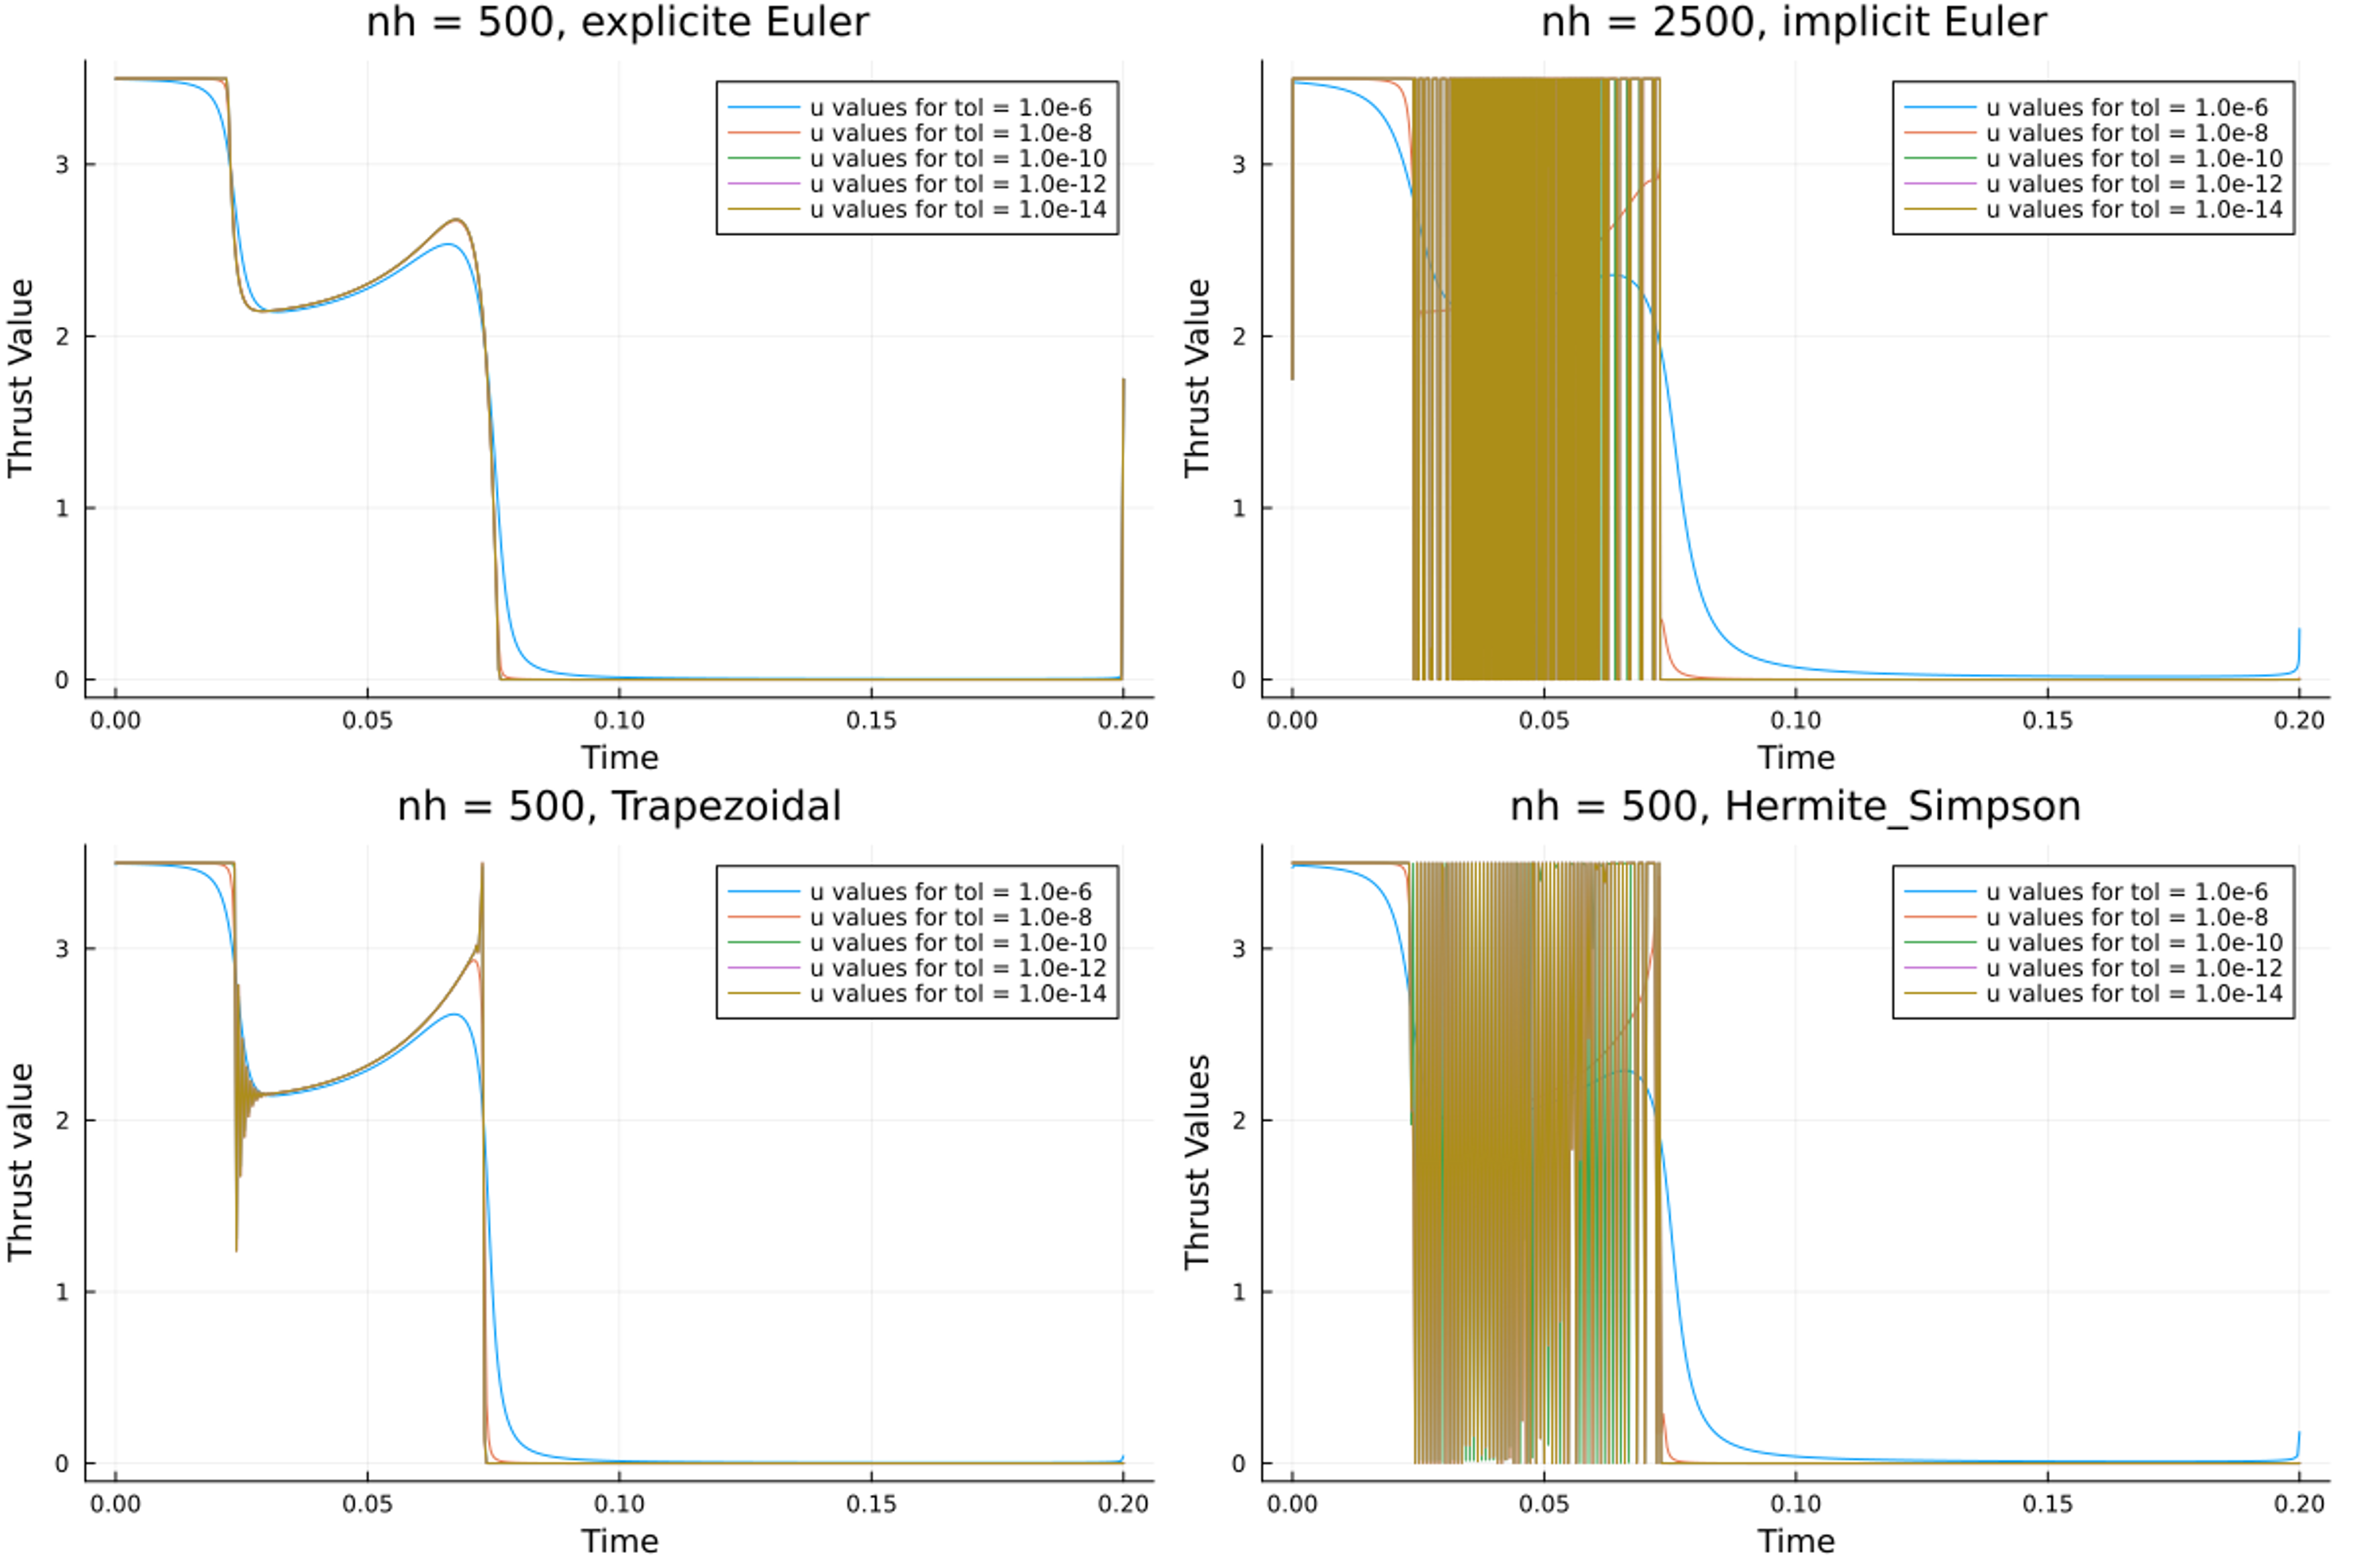
\includegraphics[width = 0.9\textwidth]{default nh.png}
    \caption{\label{fig:acceptnh} The calculated numerical solutions by different schemes of discretisation. Acceptable $nh$ and $tol$ vary from $10^{-6}$ to $10^{-14}$.}
\end{figure}

From Figure \ref{fig:acceptnh}, we concluded another common trend that with a lower tolerance, which means a higher precision, the solutions converge to the theoretical optimal solution and generate fluctuations at the same time. 

In order to further study the cause of these fluctuations appeared on the singular arc. We respectively calculated the respective eigenvalues of the reduced Hessian in function of $nh$ in Figure \ref{fig:eig}.
\begin{figure}[ht]
    \centering
    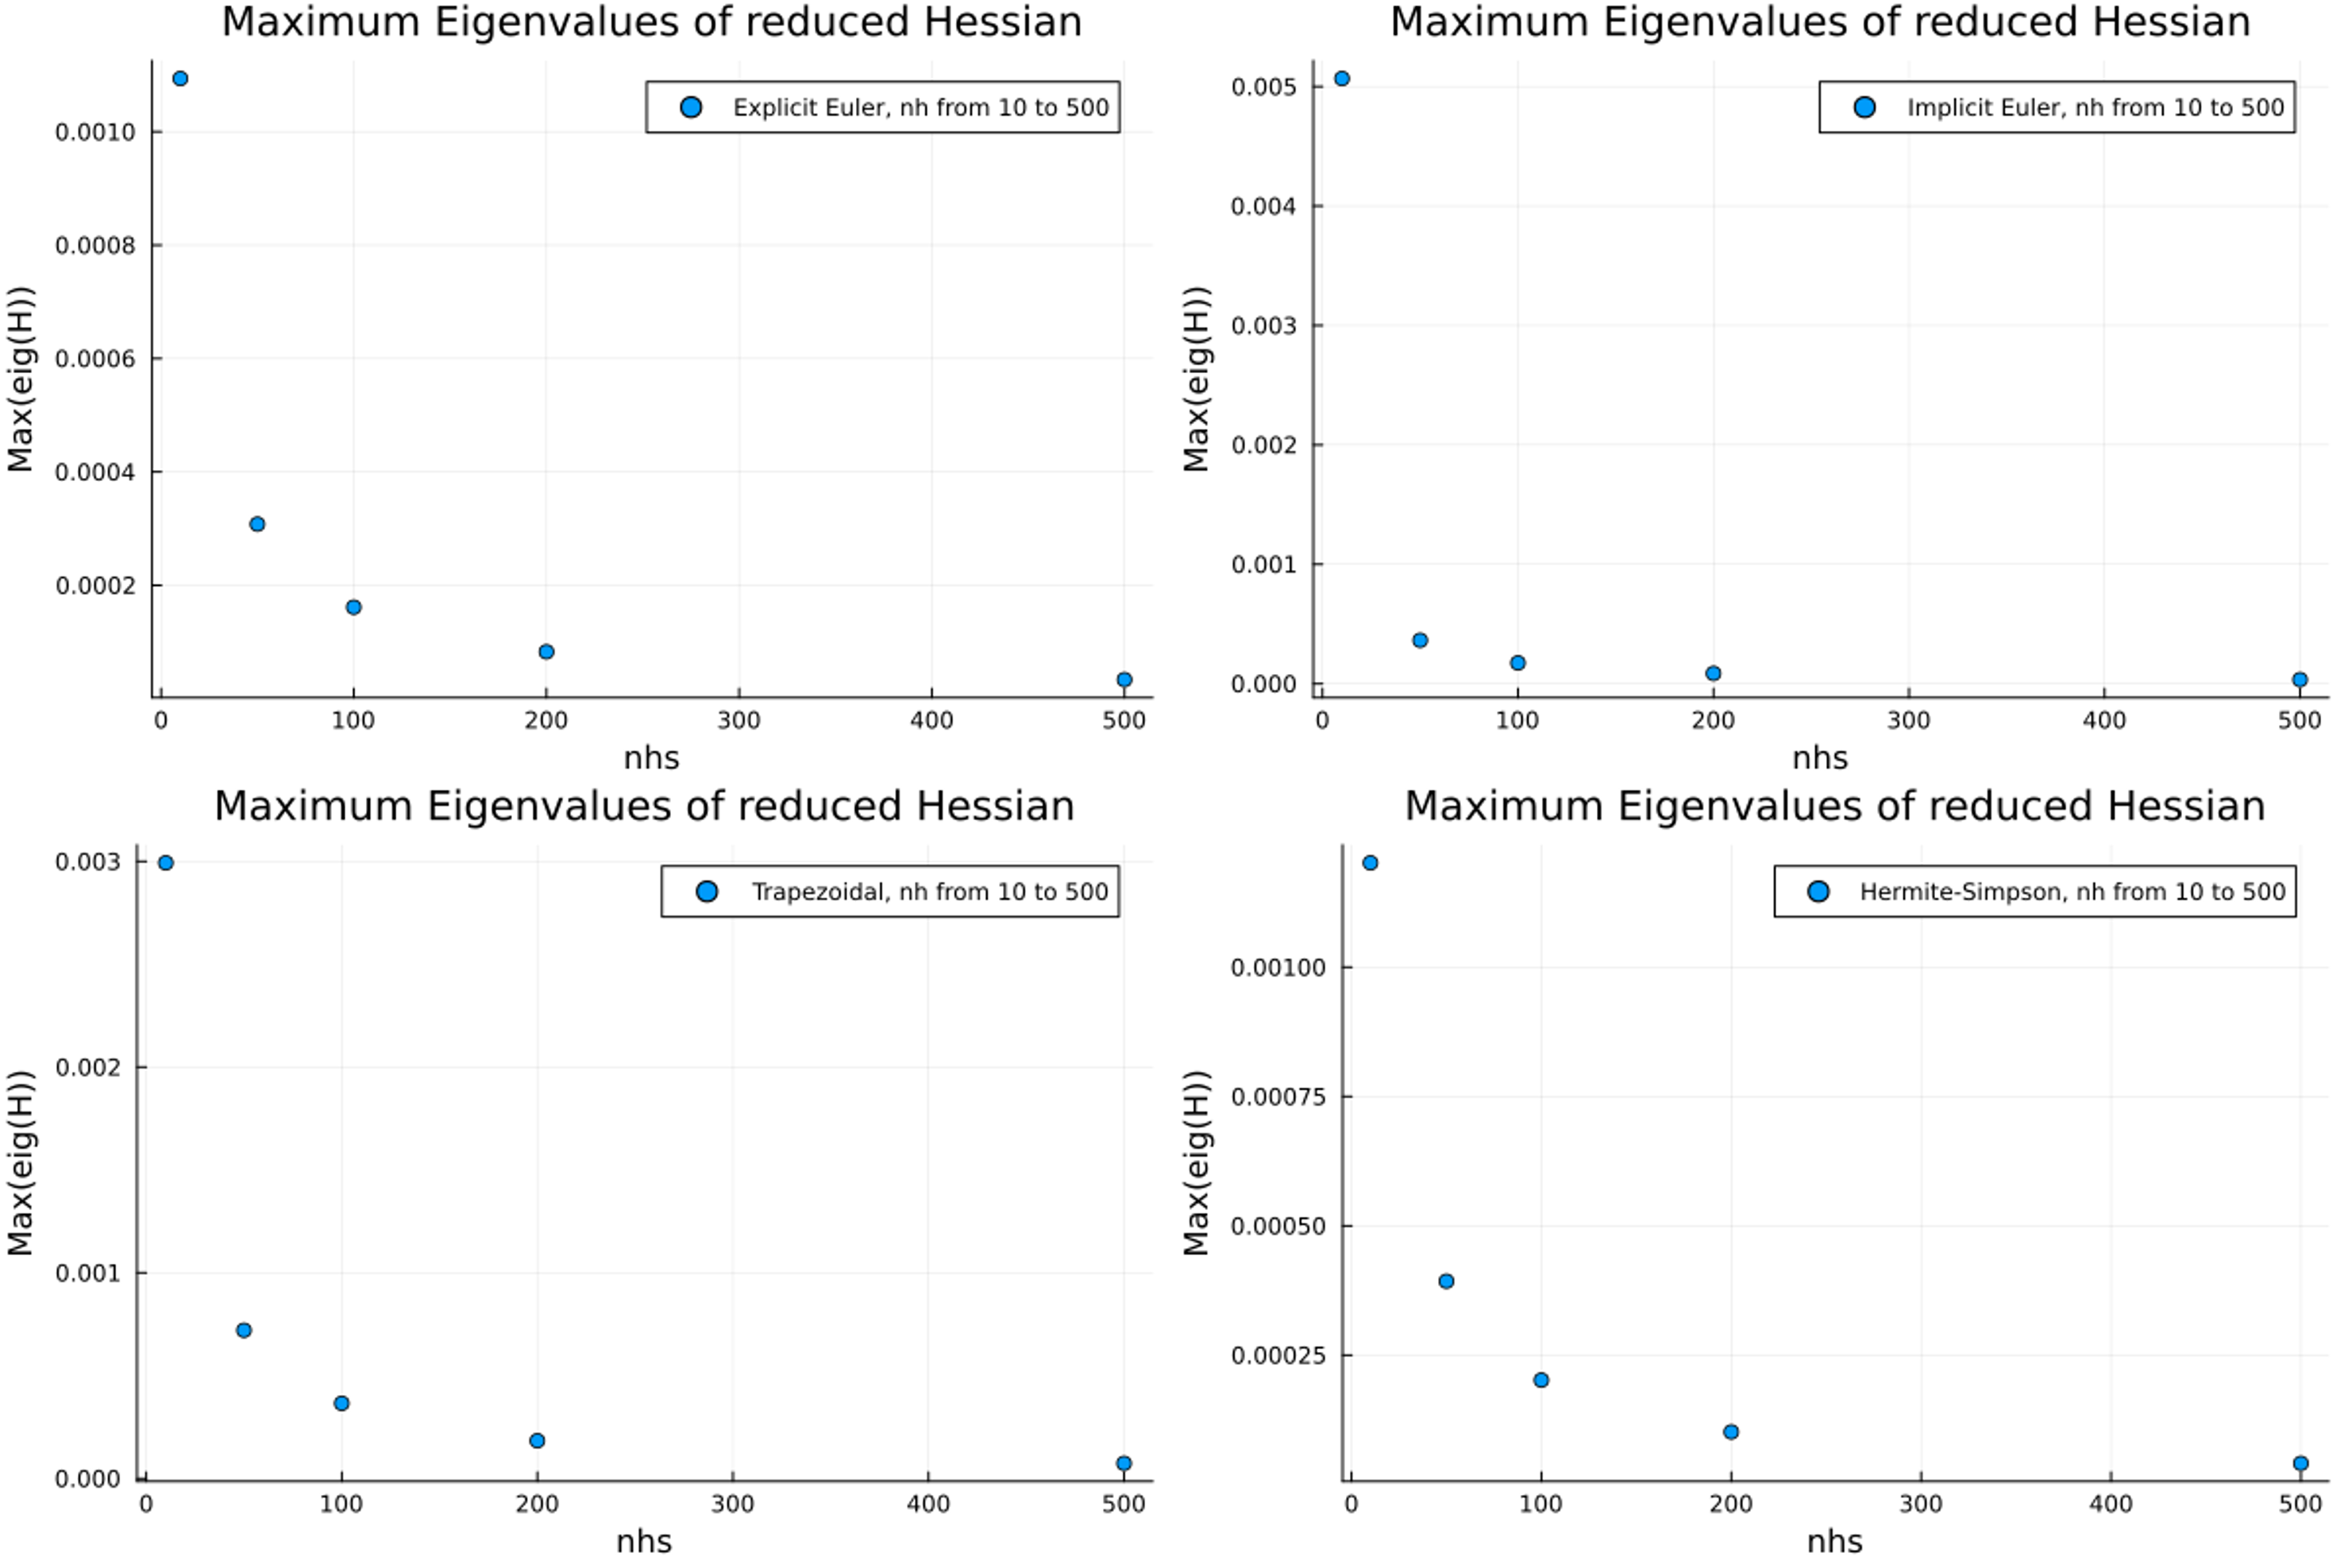
\includegraphics[width = 0.9\textwidth]{maximum eig_nh.png}
    \caption{\label{fig:eig} The maximum eigenvalues of each schemes of discretisation in function of $nh$}
\end{figure}

From Figure \ref{fig:eig}, it is clearly shown that the eigenvalues of reduced Hessian tend towards 0 when $nh$ increases. This trend indicates that the convexity of the optimal control problem reduces when a higher precision is demanded. This result guide us to look into the necessary conditions of Goddard problem discussed in section \ref{sec:NuS}. In the next section, we link the fluctuations to a failure in SOSC condition by theoretical demonstration.

\subsection{Theoretical demonstration}
In this section, we demonstrate that Goddard problem asymptotically doesn't satisfy SOSC, which means, the eigenvalues of reduced Hessian are no longer all positive. 

The proof is done in the following steps: First, we elaborate a simple case with $nh=3$, using explicit Euler scheme, where the asymptotical unsatisfaction of SOSC can be clearly concluded. Second, we generalize the case with a higher $nh$ to see whether the first proof is applicable. At last, we present the obtained solutions in different schemes of discretisation to show a generalization and consistency of this proof.
\subsubsection{Case with $nh=3$}\label{ssc:nh3}
A general numerical optimization problem with $nh=3$ realized by explicit Euler scheme is discribed as follows:
\[
\begin{aligned}
\min \  &c(x,u,\Delta) \\ 
s.t. \ &\mathbf{g}(x,u,\Delta) = 0 \\
&\underline u \le u \le \overline u
\end{aligned}
\]
where
\[
\begin{aligned}
x &= [x_0,x_1,x_2]^T \in \mathbb{R}_{3\times n_x} \\
u &= [u_0,u_1]^T \in \mathbb{R} _{2\times n_u}\\ 
\mathbf{g}_0 &= x_0 - x_{t = 0}^{ref} \\ 
\mathbf{g}_1 &= x_1 - x_0 - \Delta f(x_0,u_0) =x_1 - x_0 - \Delta f_0\\ 
\mathbf{g}_2 &= x_2 - x_1 - \Delta f(x_1,u_1) =x_2 - x_1 - \Delta f_1\\ 
\end{aligned}
\]
where $f$ is the dynamics of the system, $f: (x_n,u_n)\mapsto \dot{x}_n$. $n_x,n_u$ indicate respectively the dimension of parameters and controls.

In order to calculate the reduced Hessian, we write the Lagrangian  $ \mathcal L(x,u,\Delta)$ and the Jacobian $G$ as follows:

\[
\begin{aligned}
\mathcal{L}(x,u,\Delta) &=  c(x,u,\Delta)+ \lambda_0 \mathbf{g}_0+\lambda_1 \mathbf{g}_1+\lambda_2 \mathbf{g}_2 \\ 
\text{d} \mathbf{g} &= G_x x + G_u u + G_\Delta \Delta = G[x,u,\Delta]^T
\end{aligned}
\]

Then, 
\[
\begin{aligned}
G_x = \left[ \begin{matrix} \nabla_x\mathbf{g}_0 \\\nabla_x\mathbf{g}_1 \\\nabla_x\mathbf{g}_2 \end{matrix} \right] = \left[ \begin{matrix} I & 0& 0 \\ -I - \Delta \ \nabla_{x_0}f(x_0,u_0) & I& 0  \\ 0& -I - \Delta \ \nabla_{x_1}f(x_1,u_1) & I  \end{matrix}  \right] = \left[\begin{matrix} I&0&0\\ D_0& I &0\\ 0& D_1& I  \end{matrix}\right]
\end{aligned}
\]
with
\[
D_n = -I-\Delta \nabla_{x_n}f(x_n,u_n)
\]

And in the same way, 
\[
G_u = \left[ \begin{matrix} 0 & 0 \\ -\Delta \nabla_{u_0} f_0 & 0 \\ 0 & -\Delta \nabla_{u_1}f_1\end{matrix}\right], \quad G_\Delta = \left[ \begin{matrix}0 \\ -f_0 \\ - f_1  \end{matrix} \right],\quad G = [G_x|G_u|G_\Delta]
\]

With the above expressions, the reduced Hessian is calculated in the following form:
\[
H = Z^TWZ =Z^T\left[\begin{matrix} W_{xx}&W_{xu}&W_{x\Delta} \\ W_{ux}&W_{uu} &W_{u\Delta}  \\W_{\Delta x} & W_{\Delta u}& W_{\Delta\Delta} \end{matrix}\right] Z
\]
where $W_{ij} =\nabla_i\nabla_j \mathcal{L}(x,u,\Delta) =  (W_{ji})^T$, and $GZ = \mathbf{0}$
. With $G$ explicitly presented, we have
\[
 \quad G_x^{-1} = \left[\begin{matrix} I &0&0 \\ -D_0 &I& 0 \\ D_0D_1&-D_1&I \end{matrix}\right], \ Z = \left[\begin{matrix} -G_x^{-1} G_u& -G_x^{-1}G_\Delta \\ I&0 \\ 0&I  \end{matrix} \right]
\]

And by calculating $W$, we obtain
\[
W_{x} = \left[\begin{matrix} \lambda_0 +\lambda_1D_0 \\ \lambda_1+\lambda_2D_1 \\ \lambda_2 \end{matrix}\right]  ,\quad 
W_{xx} = \left[\begin{matrix} \lambda_1\nabla_xD_0&0&0\\0 &\lambda_2\nabla_xD_1&0\\0&0&0\end{matrix}\right],\quad W_{xu} = \left[ \begin{matrix} \lambda_1\nabla_uD_0&0\\0&\lambda_2\nabla_uD_1 \\ 0&0\end{matrix}\right]
\]

\[
W_{x\Delta}=\left[\begin{matrix}\lambda_1 \frac{\partial D_0}{\partial \Delta}\\ \lambda_2 \frac{\partial D_1}{\partial\Delta} \\ 0 \end{matrix}\right]
=\left[\begin{matrix}-\lambda_1\nabla_{x_0}f_0 \\ -\lambda_2\nabla_{x_1}f_1 \\ 0 \end{matrix}\right],\ W_{u\Delta}=\left[\begin{matrix}\lambda_1 \nabla_{u_0}f_0\\ \lambda_2 \nabla_{u_1}f_1\end{matrix}\right] 
,\ W_{uu} = W_{xx} = \mathbf{0}
\]

Then 
\[
\begin{aligned}
H &= Z^TWZ = \left[ \begin{matrix}-G_u^TG_x^{-T}&I&0 \\-G_\Delta^TG_x^{-T} &0&I \end{matrix}\right] \left[\begin{matrix} -W_{xx}G_x^{-1}G_u+W_{xu} & -W_{xx}G_x^{-1}G_\Delta+W_{x\Delta}\\-W_{xu}^TG_x^{-1}G_u &-W_{xu}^TG_x^{-1}G_\Delta +W_{u\Delta} \\ -W_{x\Delta}^TG_x^{-1}G_u +W_{u\Delta}^T & -W_{x\Delta}^TG_x^{-1}G_\Delta \end{matrix}\right] \\&=
\left[ \begin{matrix} 
G_u^TG_x^{-T}W_{xx}G_x^{-1}G_u- (A_{xu}+A^T_{xu}) 
& B
\\ B^T &G_\Delta^TG_x^{-T}W_{xx}G_x^{-1}G_\Delta-(A_{x\Delta}+A_{x\Delta}^T) 
\end{matrix}\right] \\
& = \left[\begin{matrix}
H_{11} & H_{12} \\
H_{21} & H_{22}
\end{matrix}\right]
\end{aligned}
\]
with 
\[
\begin{aligned}
A_{xu}=G_u^TG_x^{-T}W_{xu},\quad A_{x\Delta}=G_\Delta^TG_x^{-T}W_{x\Delta}\\
B = G_u^TG_x^{-T}W_{xx}G_x^{-1}G_\Delta -G_u^TG_x^{-T}W_{x\Delta}-W^T_{xu}G^{-1}_xG_\Delta+W_{u\Delta}
\end{aligned}
\]

After further calculation, we have:
\[
\begin{aligned}
H_{11} &= -\lambda_2 \Delta^2 \left[\begin{matrix}
\Delta \nabla _{x_1} f_1 (\nabla_{u_0}f_0)^2 & \nabla_{u_0}f_0\nabla_{u_1}f_1 \\
\nabla_{u_0}f_0\nabla_{u_1}f_1 & \mathbf{0}
\end{matrix} \right] \\ 
H_{12} &= B = 
\Delta \left[\begin{matrix}
    (\nabla_{u_0}f_0) f_0 - D_1 (\nabla_{u_1}f_1)f_1 - (\nabla_{u_0}f_0) D_1f_1 \\
    (\nabla_{u_1}f_1)f_1
\end{matrix}\right]
\\ &- \Delta \left[ \begin{matrix}
    \lambda_2 \nabla_{u_0}f_0 \nabla_{x_1}f_1 \\ \mathbf{0}
\end{matrix}\right]
+\Delta\left[\begin{matrix}
    \mathbf{0} \\ \lambda_2(\nabla{u_1}f_1)f_0    
    \end{matrix} \right]+\left[\begin{matrix}
        \lambda_1\nabla_{u_0}f_0 \\ \lambda_2\nabla_{u_1}f_1
    \end{matrix}\right]
\\
H_{22} &= \Delta \left[\begin{matrix}
    \lambda_1 & \lambda_2
\end{matrix}\right]
\left[\begin{matrix}
    (f_0D_0-f_1D_0D_1)^T\nabla_{x_0}f_0(f_0D_0-f_1D_0D_1)  \\ (f_1D_1-f_0)^T\nabla_{x_1}f_1(f_1D_1-f_0)
\end{matrix}\right]
\end{aligned}
\]

From these calculations, we can conclude that most part of the reduced Hessian ($H_{11}\in\mathbb{R}_{n_u\times n_u}$) follows the nature of $H_{11}\sim O(\Delta^2)$, and the rest of the reduced Hessian ($H_{22}\in\mathbb{R}_{1\times1}$) follows the nature of $H_{22}\sim O(\Delta)$. Which indicates that asymptotically, all the values of reduced Hessian tends towards 0 and thus, the eigenvalues are no longer all positive. The SOSC is asymptotically unsatisfied.

\subsubsection{Generalization of the $nh$}

When redoing the proof of the \ref{ssc:nh3} with a higher $nh$, we need to prove the invertibility of $G_x$ for any $nh$. For a given nh, we have:

\[
G_x = \left[\begin{matrix}
    I & 0 & 0 &\cdots & 0 & 0\\
    D_0 & I & 0 & \cdots & 0 & 0 \\
    0 & D_1 & I & \cdots & 0 & 0 \\
    \vdots & \vdots &\vdots  &\ddots &\vdots &\vdots \\
    0 & 0 & 0 &\cdots & D_{nh-2} & I
\end{matrix} \right]\in \mathbb{R}_{(n_x\times nh)\times(n_x\times nh)}
\]

To calculate this determinant, we notice that $G_x$ is a lower triangular matrix with all diagonal terms equal to 1, which directly indicates that $det(G_x)=1$. 
We can conclude that $G_x$ is invertible for any given $nh$.

\subsubsection{Consistency in different schemes of discretisation}
This section show the numerical results to verify the trends we concluded in section\ref{ssc:nh3}. We ought to observe the following phenomenons: 
\begin{itemize}
    \item The maximum term of the reduced Hessian scales proportionally to $\Delta^2$, which is $\frac{1}{nh^2}$
    \item The maximum eigenvalues of the reduced Hessian tends to zero when $nh$ tends to infinity
\end{itemize}

And the results of numerical calculations are as follows: Figure \ref{fig:maxH} shows the trends that the maximum term of the reduced Hessian tends to 0 on the order of $\Delta^2$,Figure \ref{fig:maxeig} shows the trends that the maximum eigenvalues tends to 0 when nh tends to infinite, which indicates the asymptotical unsatisfaction of SOSC. 

\begin{figure}[ht]
    \centering
    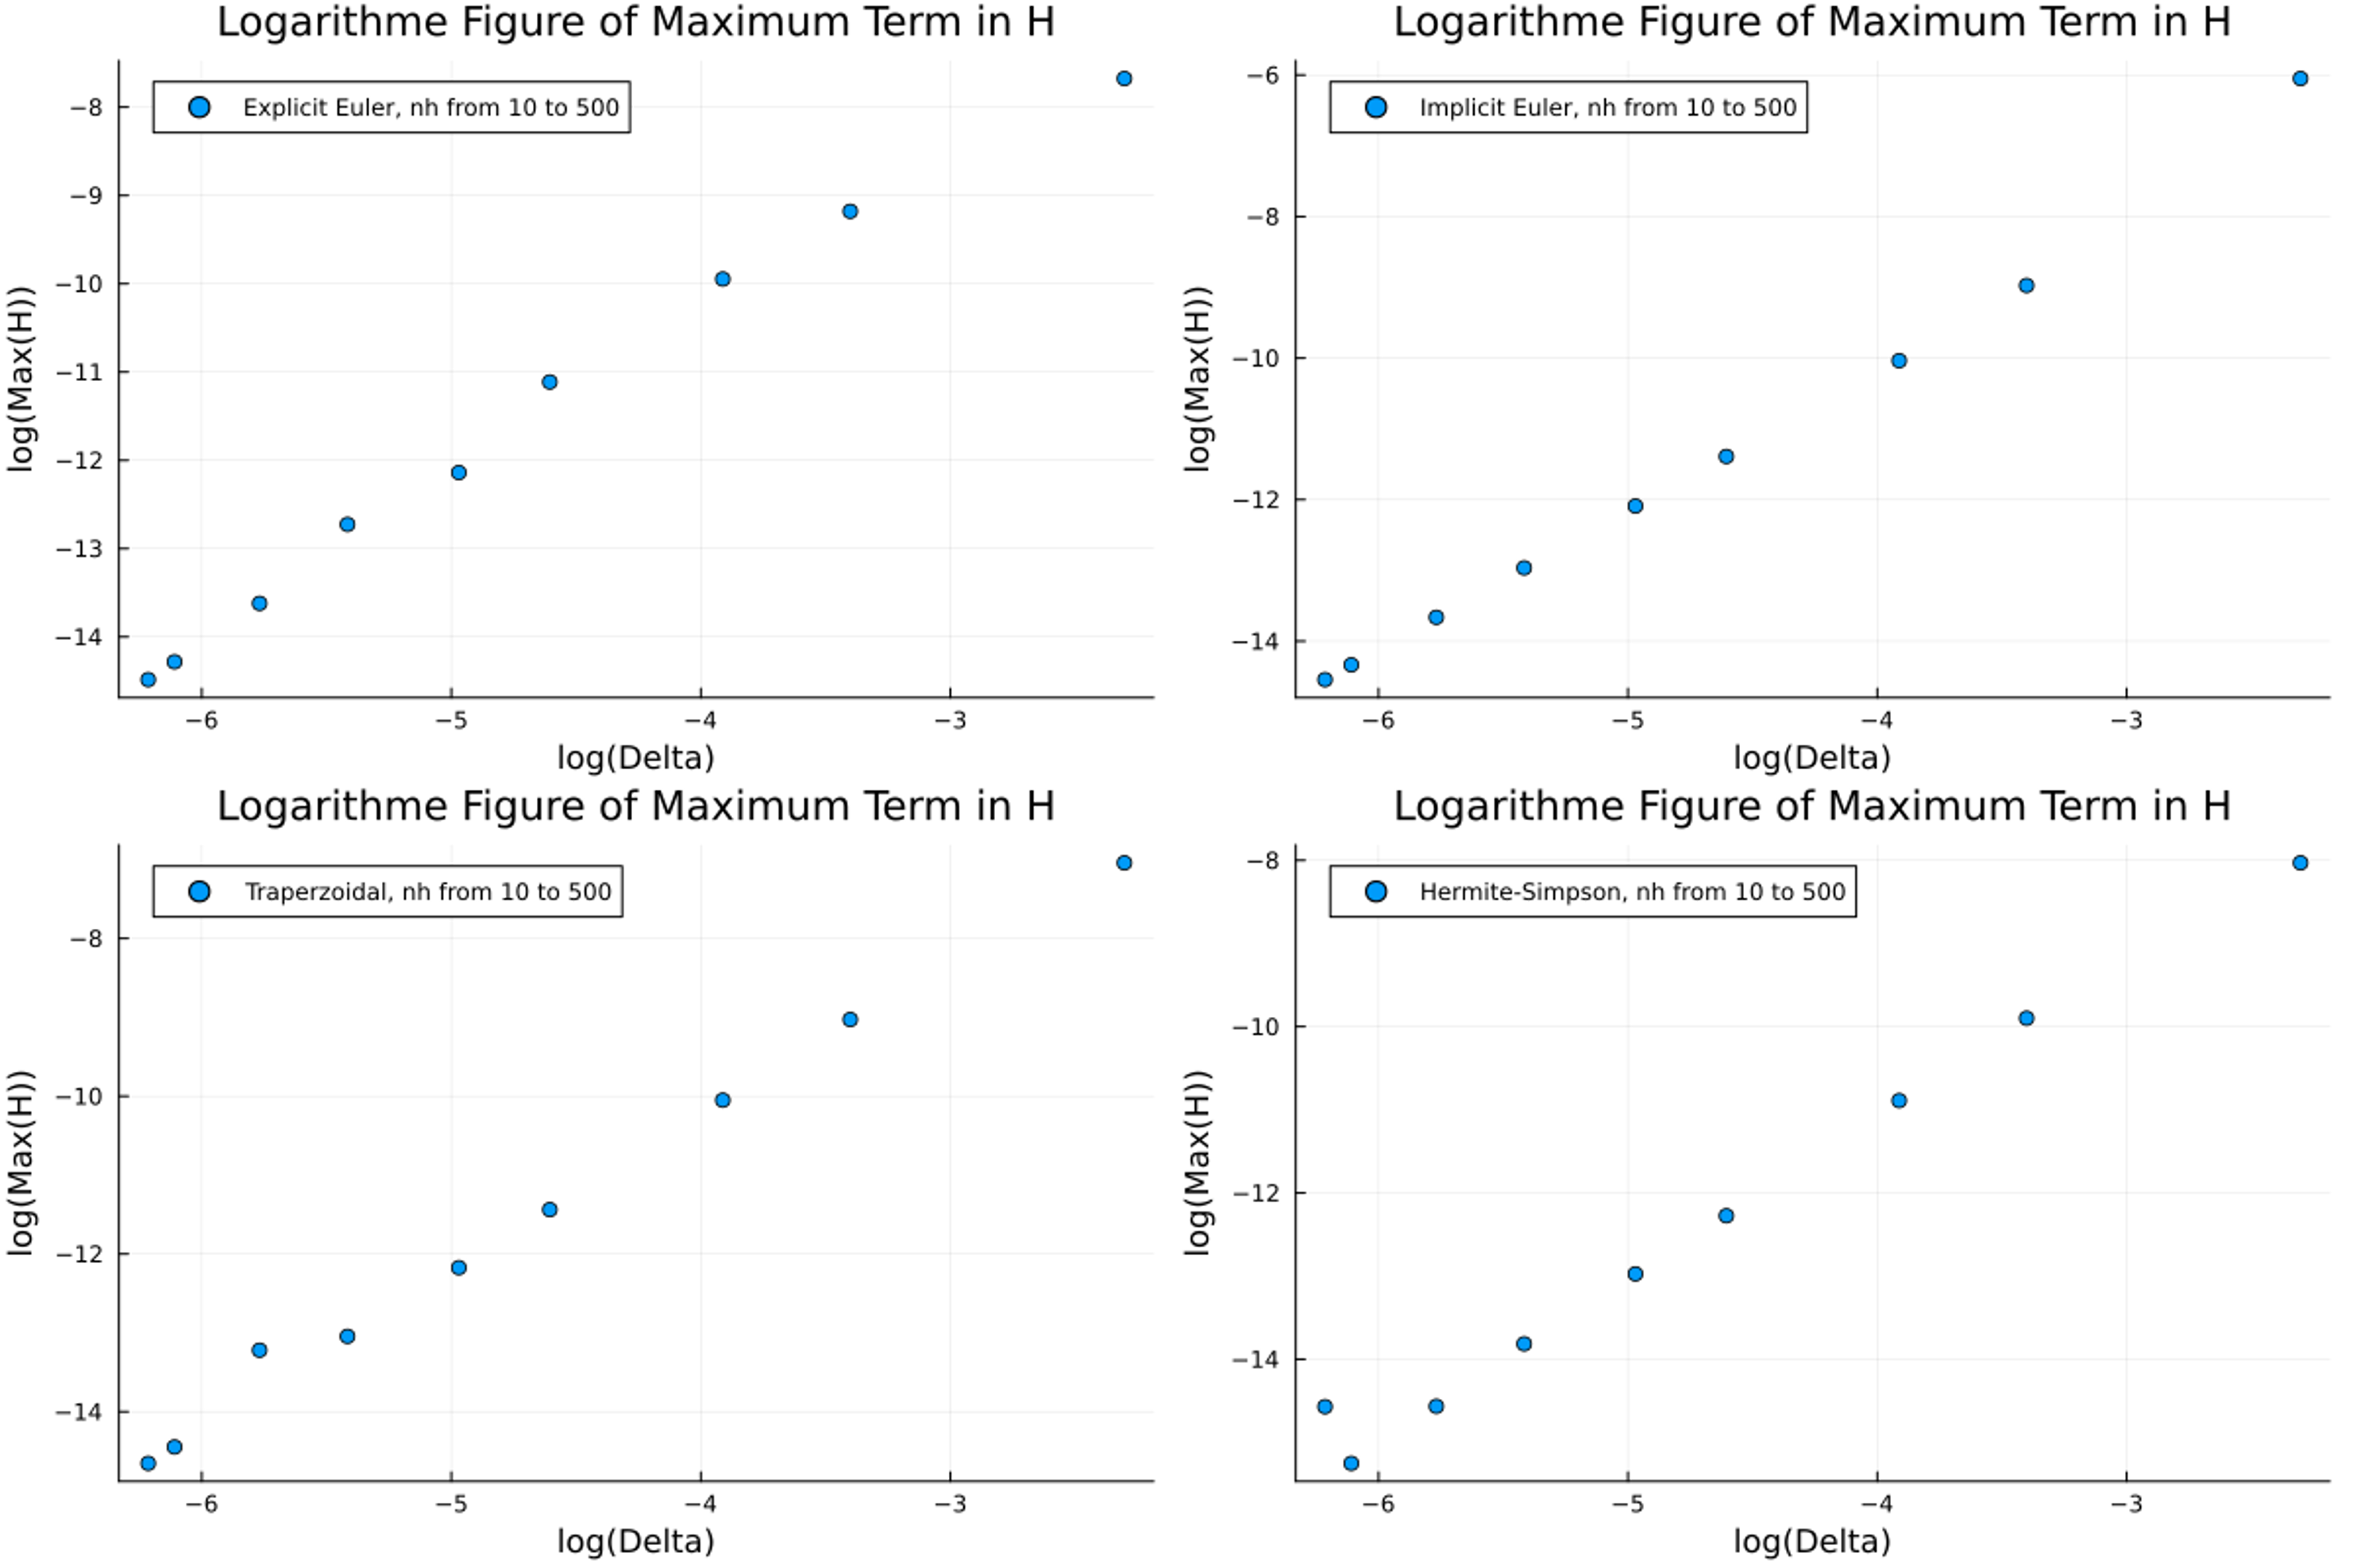
\includegraphics[width = \textwidth]{Log_maxH.png}
    \caption{\label{fig:maxH} The calculated maximum terms of main part of reduced Hessian $H_{11}$ with nh vary from 10 to 500}
\end{figure}

\begin{figure}[ht]
    \centering
    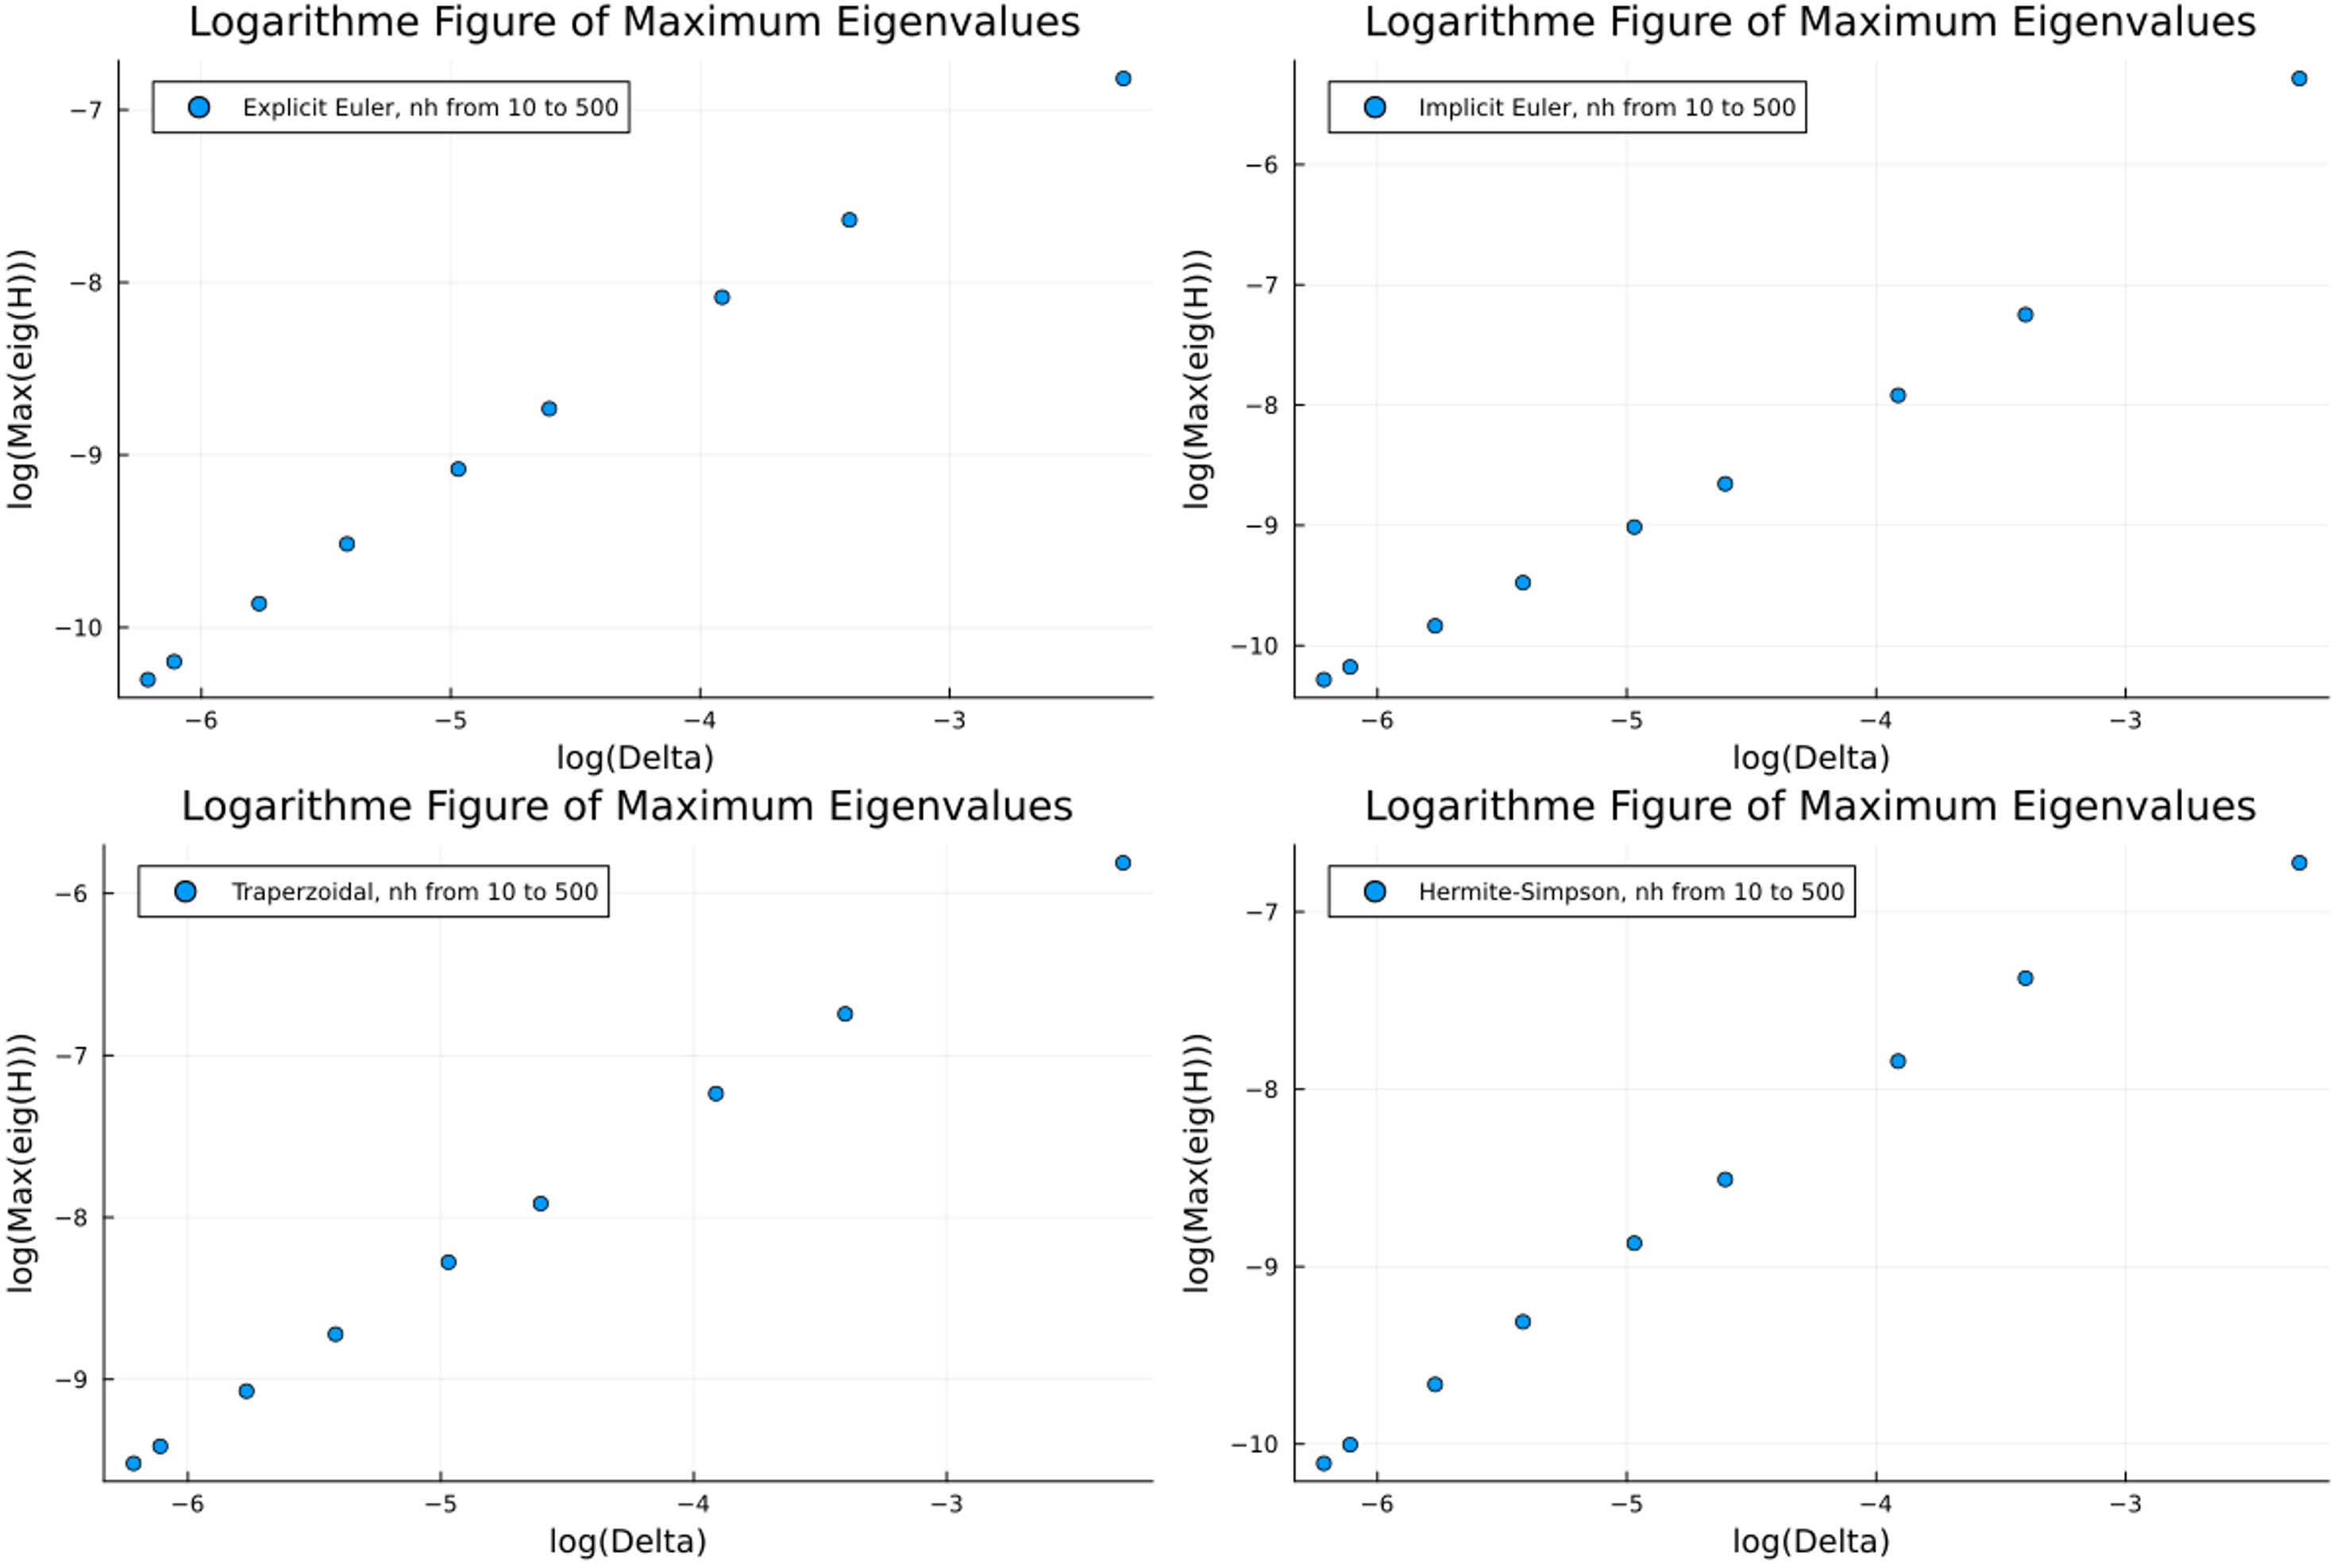
\includegraphics[width = \textwidth]{Log_maxEig.png}
    \caption{\label{fig:maxeig} The calculated maximum terms of main part of reduced Hessian $H_{11}$ with nh vary from 10 to 500}
\end{figure}

The above results not only show the behavior of the reduced Hessian as nh increases, where the slope of $Max(H)$ over $\log(\Delta)$ corresponds very well to the theoretical demonstration, but also show a consistency between different schemes of discretisation, which indicates that the demonstration in \ref{ssc:nh3} is generalizable.

With all the above demonstration, we prove the unsatisfaction of SOSC in Goddard problem. This demonstration helps us to improve the accuracy of numerical solutions from the perspective that we need to increase the local convexity to satisfy SOSC.
\subsection{Improvements made by integrated residuals}
\label{sec:Imp}
One of the imporvements to avoid fluctuations made by Yuanbo Nie and Eric C. Kerrigan\cite{Solving Dynamic Optimization} is to add a penalty term to the final optimization objective, named integrated residuals. This penalty reduces the sudden changes in control $u$ by closing the solution to an explicit Euler solution, where the fluctuations only appears when $nh$ is extremely high. The integrated residual is calculated as follows:

\[
\begin{aligned}
    &\min_{u}\int_0^{t_f}\|\epsilon(t)\|_{2}dt \\
    &\epsilon(t)=\left[\begin{matrix}
        \dot{x}(t)-f(x(t),u(t)) \\ h(x(t),u(t))
    \end{matrix}\right]
\end{aligned}
\]
where $f$ is the dynamics of the system and $h$ represent the equality constraints of the system.

In this research, we established a weight coefficient named $w_{obj}$, to balance the weight of initial objective and the integrated residual. The new optimization objective is defined as follows:
\[
\begin{aligned}
    &\min_{u}\int_0^{t_f}w_{e}\|\epsilon(t)\|_{2}dt - w_{obj}h(t_f) \\
    &w_{e}+ w_{obj}=1
\end{aligned}
\]
where $w_{e}$ and $w_{obj}$ are coefficients vectors of corresponding dimensions, calculated by weighted average of $h_0$, $m_0$ and $\Delta g_0$. Thus, when $w_{obj}=1$, the new objective is identical to the original one. When $w_{obj}=0$, the model is set to only satisfy the dynamics of the system, while not maximizing the final height.

The improvements of obtained with the integrated residual and the weight coefficient into the original model are shown in the following comparisons:
\begin{figure}[ht]
    \centering
    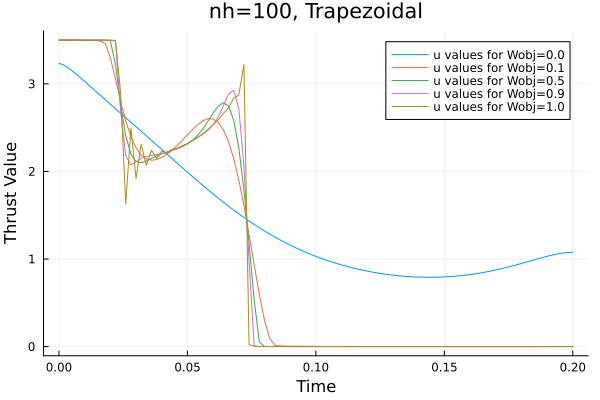
\includegraphics[width = \textwidth]{obj_trap.png}
    \caption{\label{fig:obj_trap} Numerical solutions realized by Trapezoidal discretisation}
\end{figure}

\begin{figure}[ht]
    \centering
    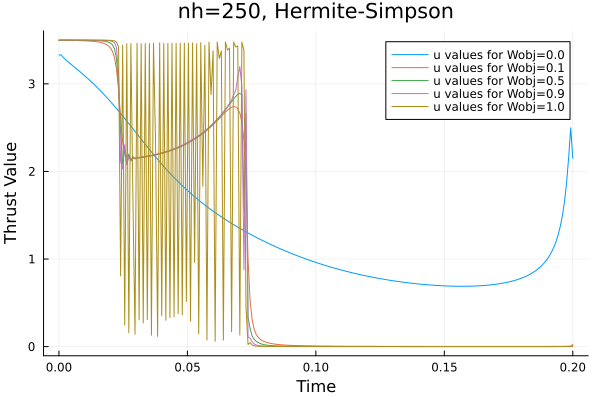
\includegraphics[width = \textwidth]{obj_hersim.png}
    \caption{\label{fig:obj_hersim} Numerical solutions realized by Trapezoidal discretisation}
\end{figure}

The Figure \ref{fig:obj_trap} shows that, compared to the original solution (presented in brown-yello curve), the weighted-integrated residual method eliminates the fluctuations at the beginning and at the end of singular arc. With a good choice of $w_{obj}$, in this case the purple-pink curve, the new method will neither generate fluctuations nor over-smoothen the peak in the optimal solution.

The improvements given by the weighted integrated residual is more clearly presented in Figure \ref{fig:obj_hersim}, where a significant improvement of precision is observed by tuning $w_{obj}$ to 0.9. As comparison, the similar quality of solution is only obtained with $nh=500$ using the original optimization model.
\clearpage

\section{Conclusion}
\subsection{High precision solution of Goddard problem}
This research focus on obtaining high precision solutions of Goddard problem, the findings are as follows:
\begin{itemize}
    \item When calculating numerical solutions of Goddard problem, simply increasing the number of discretisation or lowering the tolerance doesn't necessarily returns solution of higher quality, especially considering the optimization behavior on the singular arc. To be specific, an overly big number of discretisation returns solutions with over smoothened peak at the end of the singular arc, while a small number of discretisation or an overly low tolerance generates fluctuations on the singular arc. 
    \item The cause of the lack of precision is, at least partly, an asymptotical unsatisfaction of SOSC when nh increases. With theoretical demonstration and verification of numerical calculation results, the terms of reduced Hessian are proven to tend towards zero on the order of $\frac{1}{nh^2}$, which causes the eigenvalues to no longer be all positive.
    \item To add convexity to the optimization model and eliminate the appeared fluctuations when number of discretisation is low, a weighted integrated residual method, based on integrated residual method, is proposed and verified in this research. With a good choose of weight coefficient, usually near 1, a high precision solution can be calculated with relatively lower nh. This method helps to fulfill the need of a high precision solution within reasonable computational resource while avoiding the generated fluctuations.
\end{itemize}
\subsection{Summary of conducted works}
During this research, the main personal contributions are as follows:
\begin{itemize}
    \item Integration of different schemes of discretisation into the JuMP optimization models.
    \item Generation and analysis of the numerical solutions under different sets of parameters, variables and models.
    \item Theoretical demonstration of the lack of SOSC in Goddard problem, especially the part of matrix calculations.
    \item Realization of integrated residual method and modificating it into weighted integrated residual to better fit the need of precision.
\end{itemize}
The scripts and generated photos in this research are available on Github, URL:https://github.com/MaloZHOU/TR-Contr-le-Multi-Pr-cision-ZHOU
\subsection{Shortcomings in this research}
It is important to mention that this research is still facing with the following limitations and shortcomings:
\begin{itemize}
    \item Due to the personal limitations of coding capability, I haven't realized other schemes of discretisation, especially the 4-Runge-Kutta method. This shortcoming limits the universalization of the conclusion.
    \item Due to the complexity of optimization progress and difference between solvers and schemes, we haven't considered a better criteria of "computational resource" except for the number of discretisation. One of the ideal analysis of computational resource is to calculate the spatial complexity and time complexity, which can be another topic to study on.
    \item Although the numerical results show consistency between schemes of discretisation, some parts of calculation in the demonstration may change and lead to different result when using different schemes of discretisation.
\end{itemize}
\clearpage

\begin{thebibliography}{99}
    \bibitem{A method of reaching}
    Robert H. Goddard,
    \textit{A Method of Reaching Extreme Altitudes},
    volume 71(2) of Smithsonian Miscellaneous Collections. Smithsonian institution, City of Washington, 1919.
    
    \bibitem{Betts}
    Betts, John T.
    \textit{Practical Methods for Optimal Control and Estimation Using Nonlinear Programming,  Second Edition},
    Society for Industrial and Applied Mathematic, 2010.
    
    \bibitem{Bryson}
    Bryson, A.E.
    \textit{Applied Optimal Control: Optimization, Estimation and Control}
    Routledge, 1975.
    
    \bibitem{Solving Dynamic Optimization}
    Nie, Yuanbo and Kerrigan, Eric C.
    \textit{Solving Dynamic Optimization Problems to a Specified Accuracy: An Alternating Approach Using Integrated Residuals}
    IEEE Transactions on Automatic Control, vol. 68, no. 1, pp. 548-555, Jan. 2023.
\end{thebibliography}


\end{document}
